%%%%%%%%%%%%%%%%%%%%%%%%%%%%%%%%%%%%%%%%%
% University Assignment Title Page 
% LaTeX Template
% Version 1.0 (27/12/12)
%
% This template has been downloaded from:
% http://www.LaTeXTemplates.com
%
% Original author:
% WikiBooks (http://en.wikibooks.org/wiki/LaTeX/Title_Creation)
%
% License:
% CC BY-NC-SA 3.0 (http://creativecommons.org/licenses/by-nc-sa/3.0/)
% 
% Instructions for using this template:
% This title page is capable of being compiled as is. This is not useful for 
% including it in another document. To do this, you have two options: 
%
% 1) Copy/paste everything between \begin{document} and \end{document} 
% starting at \begin{titlepage} and paste this into another LaTeX file where you 
% want your title page.
% OR
% 2) Remove everything outside the \begin{titlepage} and \end{titlepage} and 
% move this file to the same directory as the LaTeX file you wish to add it to. 
% Then add \input{./title_page_1.tex} to your LaTeX file where you want your
% title page.
%
%%%%%%%%%%%%%%%%%%%%%%%%%%%%%%%%%%%%%%%%%
%\title{Title page with logo}
%----------------------------------------------------------------------------------------
%	PACKAGES AND OTHER DOCUMENT CONFIGURATIONS
%----------------------------------------------------------------------------------------
\documentclass[12pt]{article}
\usepackage[spanish, es-tabla]{babel}
\usepackage[utf8x]{inputenc}
\usepackage{amsmath}
\usepackage{graphicx}
\usepackage[colorinlistoftodos]{todonotes}
\usepackage{makeidx}
\usepackage[colorlinks=true,linkcolor=black,anchorcolor=black,citecolor=black,filecolor=black,menucolor=black,runcolor=black,urlcolor=blue]{hyperref}
\usepackage{color}
\usepackage{caption}
\usepackage{etoolbox}
\usepackage{fancybox}
\usepackage{enumitem}
\usepackage{listings}
\lstset{
	language=sh,
	breaklines=true,
	breakatwhitespace=true,
	basicstyle=\ttfamily,
	showstringspaces=false,
	columns=fullflexible-
}
\usepackage{booktabs}
\usepackage{tabularx}
\usepackage{lipsum}
\usepackage{multirow}

\newcommand\pro{\item[$+$]}
\newcommand\con{\item[$-$]}

\newcommand{\icon}[1]{\includegraphics[height=18pt]{#1}}
\robustify{\icon}
\makeindex
\graphicspath{{./img/}}

\begin{document}

\renewcommand\indexname{Índice}
\begin{titlepage}

\newcommand{\HRule}{\rule{\linewidth}{0.5mm}} % Defines a new command for the horizontal lines, change thickness here

\center % Center everything on the page
 
%----------------------------------------------------------------------------------------
%	HEADING SECTIONS
%----------------------------------------------------------------------------------------

\textsc{\LARGE Facultad de Informática}\\[1.5cm] % Name of your university/college
\textsc{\large Adrián García García}\\[0.5cm] % Minor heading such as course title

%----------------------------------------------------------------------------------------
%	TITLE SECTION
%----------------------------------------------------------------------------------------
\newcommand*{\TitleFont}{%
      \usefont{\encodingdefault}{\rmdefault}{b}{n}%
      \fontsize{19}{23}%
      \selectfont}


\HRule \\[0.4cm]
{ \TitleFont \bfseries Instrumentación del runtime de OpenMP}\\[0.4cm] % Title of your document
\HRule \\[1.5cm]
 
%----------------------------------------------------------------------------------------
%	AUTHOR SECTION
%----------------------------------------------------------------------------------------


% If you don't want a supervisor, uncomment the two lines below and remove the section above
%\Large \emph{Author:}\\
%John \textsc{Smith}\\[3cm] % Your name

%----------------------------------------------------------------------------------------
%	DATE SECTION
%----------------------------------------------------------------------------------------

{\large \today}\\[2cm] % Date, change the \today to a set date if you want to be precise

%----------------------------------------------------------------------------------------
%	LOGO SECTION
%----------------------------------------------------------------------------------------


\includegraphics[width=4cm,keepaspectratio]{logo.png}
 
%----------------------------------------------------------------------------------------

\vfill % Fill the rest of the page with whitespace



\captionsetup[figure]{labelformat=empty,justification=raggedright,singlelinecheck=false}
% Include image from images directory
\begin{figure}[h]

        
\includegraphics[width=2cm,keepaspectratio]{cc-by-sa.png}
        \label{fig:by-sa}
        \caption{ This work is licensed under a \href{https://creativecommons.org/licenses/by/4.0/legalcode}{CC-BY-SA 4.0 License}.}

\end{figure}

\end{titlepage}

\tableofcontents
\clearpage



\section{Introducción}\label{sec:intro}

Este trabajo tiene como objetivo realizar una instrumentación del runtime de OpenMP para permitir la recolección de métricas de rendimiento en los programas que hacen uso de esta API de paralelización. La conferencia relacionada con este trabajo estaba orientada más hacia el paradigma de computación basado en tareas y la paralización de diferentes programas que se ejecutan en procesadores simétricos convencionales. Sin embargo, en el ámbito de investigación en el que participo junto al profesor Juan Carlos Sáez Alcaide hemos observado que la gran mayoría de benchmarks multihilo de suites comerciales (SPEC, PARSEC, Minebench, etc.) hacen uso de directivas de paralelización convencionales como \textit{\#pragma parallel for}. Con el objetivo de evaluar el rendimiento de estos benchmarks, he realizado una instrumentación del runtime de OpenMP y más adelante presentaré un caso de estudio para exponer diferentes retos que debe afrontar su runtime en sistemas multicore asimétricos (AMP). 

La parelización basada en directivas de compilación que reparten el trabajo de los bucles realiza una división del espacio de iteraciones en fragmentos de igual tamaño para cada hilo. No obstante, esta aproximación trae significativos problemas de rendimiento y justicia en los sistemas AMP, ya que sus cores funcionan a diferente frecuencia y pueden presentar características microarquitectónicas diversas (diferentes tamaños de cache, ejecución en orden o fuera de orden, etc.). Estas diferencias provocan que un hilo que se ejecuta en un core big generalmente termine antes su asignación de trabajo. Cuando sucede esto, estos hilos se suelen bloquear en una barrera de memoria a través de una espera activa con el objetivo de sincronizarse con el resto de hilos que se ejecutaban en cores small. Considero que esta situación representa un desperdicio de recursos debido a dos motivos principales:

\begin{itemize}
	\item Los sistemas operativos de propósito general no son capaces de identificar a los hilos que realizan una espera activa y, por tanto, su planificador no puede intercambiar estos hilos por otros que sean capaces de hacer un uso efectivo de los cores.
	\item En el contexto de monitorización del rendimiento y recogida de métricas para la toma de decisiones de planificación, las técnicas de espera activa como mecanismo de sincronización generan unos valores de rendimiento engañosos. Esto se debe a que los hilos que usan estas técnicas producen unos valores altos de IPC, cuando en realidad se encuentran ejecutando instrucciones inútiles para el progreso de la aplicación. Estas medidas pueden llevar a tomar decisiones erróneas al planificador o incluso a realizar cargos adicionales en plataformas de Cloud Computing en las que se factura a los usuarios en base al tiempo de uso de CPU y a diferentes métricas recogidas en tiempo de ejecución.
\end{itemize}


Con el objetivo de recoger información de diferentes métricas de rendimiento he elegido utilizar PMCTrack~\cite{pmctrack}, se trata de una herramienta de monitorización del rendimiento a través de contadores hardware para Linux. Esta herramienta ha sido diseñada especialmente para ayudar a los desarrolladores del kernel en la implementación de algoritmos de planificación que utilizen los datos de los contadores de monitorización del rendimiento (Performance Monitoring Counters - PMCs) para realizar optimizaciones en tiempo de ejecución. A pesar de ser una herramienta orientada al sistema operativo, PMCTrack también está equipada con una serie de componentes en espacio de usuario (bibliotecas, entorno gráfico y de línea de comandos) que permiten obtener información de monitorización de aplicaciones en ejecución. En este trabajo se utilizará la biblioteca de PMCTrack para instrumentar el código del runtime de OpenMP y poder recoger diferentes métricas de los bucles paralelizados con este framework. Se puede encontrar un manual de usuario junto a una guía de instalación en la página web oficial del proyecto~\cite{pmc-userguide}.
\begin{figure}[tbp]
    \centering
    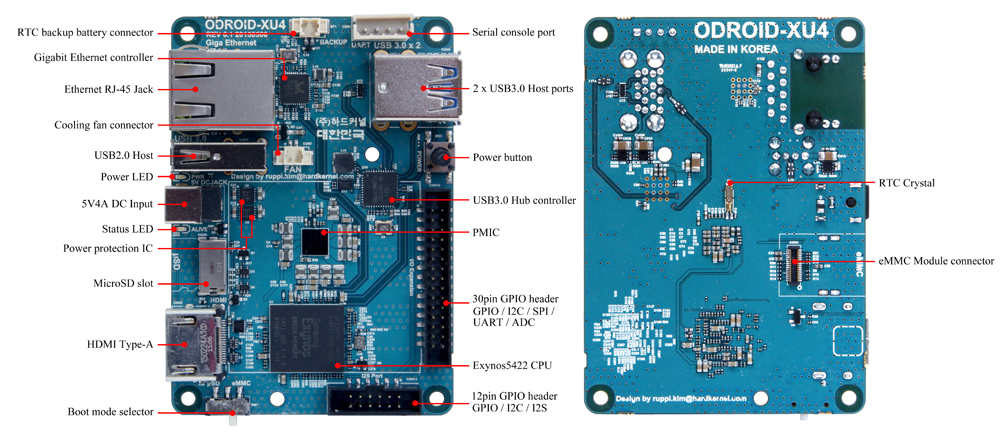
\includegraphics[width=1\textwidth]{foto_placa_XU4.png}
    \caption{Placa ODROID-XU4}
    \label{fig:fotoPlacaXU4}
\end{figure}

Para la realización de este trabajo se ha empleado la placa de desarrollo Odroid XU4~\cite{odroid-manual}, el principal motivo de su elección es que incorpora un procesador multicore asimétrico y, además, ya contaba con experiencia trabajando con ella en el Trabajo de Fin de Grado y anteriores investigaciones. Esta placa está provista de un SoC(\emph{System-On-Chip}) Exynos 5422 de Samsung fabricado en 28nm, que integra un procesador ARM big.LITTLE de ocho núcleos. Estos se dividen en dos clusters, cuatro cores Cortex A15 (2GHz) con ejecución fuera de orden y 2MB de último nivel de cache (L2) y otros cuatro cores Cortex A7 (1.4GHz) con ejecución en orden y 512KB de LLC (L2). Ambos comparten espacio de direcciones para acceder a una memoria principal DDR3 de 2GB que funciona a 750  MHz. Para mostrar la configuración de la placa con mayor detalle, la figura \ref{fig:diagramaDeBloquesXU4} muestra el diagrama de bloques de la placa Odroid XU4.


\begin{figure}[tbp]
    \centering
    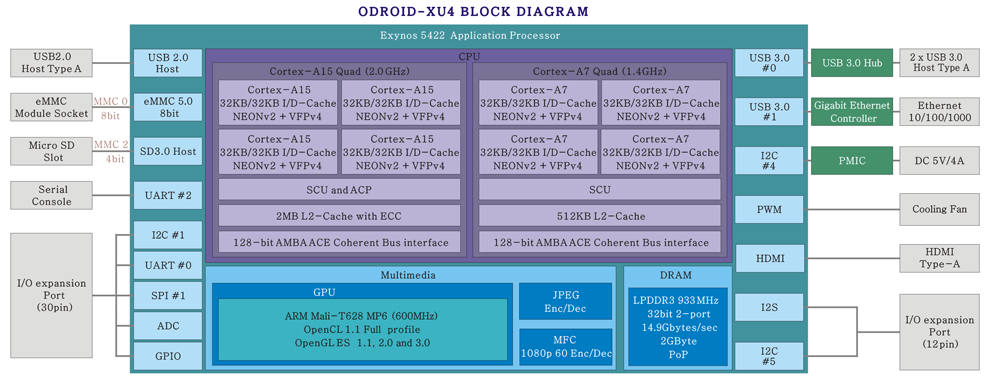
\includegraphics[width=1\textwidth]{diagrama_de_bloques_ODROID_XU4.png}
    \caption{Diagrama de bloques de la placa Odroid XU4}
    \label{fig:diagramaDeBloquesXU4}
\end{figure}


El resto del trabajo está estructurado de la siguiente forma, en la Sección~\ref{sec:expent} se describe de forma detallada el entorno experimental y los pasos seguidos para su construcción. En primer lugar, se explica cómo usar un compilador cruzado y por qué es necesario en la Sección \ref{sec:crucomp}. A continuación, en la Sección~\ref{sec:instrum} se describe el proceso seguido para instrumentar el runtime de OpenMP y en qué partes del código fue necesario introducir llamadas a la librería de PMCTrack para recoger métricas de la paralelización de bucles en tiempo de ejecución. Más adelante, en la Sección~\ref{sec:recolecc} se expone la forma de activar la instrumentación para ejecutar un benchmark y medir el rendimiento de su ejecución con diferentes métricas. Por último, en la Sección~\ref{sec:results} se presentan los resultados obtenidos al instrumentar la ejecución de benchmarks paralelos en la placa Odroid XU4 y en la Sección~\ref{sec:conclu} se exponen las conclusiones que he obtenido de este trabajo.

\section{Entorno experimental}\label{sec:expent}

\subsection{Construcción de un compilador cruzado}\label{sec:crucomp}

\subsection{Instrumentación del runtime de OpenMP}\label{sec:instrum}

En esta sección se explicará el procedimiento seguido para instrumentar el runtime de OpenMP usando la librería de PMCTrack. Con el fin de aprender a usar esta librería, se consultaron los ejemplos disponibles de forma pública junto a las fuentes del proyecto en el repositorio oficial de PMCTrack en github ~\cite{pmc-git}.

\subsection{Recolección de métricas}\label{sec:recolecc}

\section{Resultados}\label{sec:results}

\section{Conclusiones}\label{sec:conclu}


\begin{thebibliography}{1}
%\bibitem{key} description. \href{https://...}{Enlace}
\bibitem{pmctrack}\textit{An OS-oriented performance monitoring tool for multicore systems}. Saez, J. C., Casas, J., Serrano, A., Rodríguez-Rodríguez, R., Castro, F., Chaver, D., \& Prieto-Matias, M. (2015, August). In European Conference on Parallel Processing (pp. 697-709). Springer International Publishing.
\bibitem{pmc-git} \textit{Repositorio oficial de PMCTrack}. Ejemplos de código utilizados disponibles en \textit{pmctrack/test/test\_libpmctrack/}. \href{https://github.com/jcsaezal/pmctrack}{Enlace a git}.
\bibitem{pmc-userguide} \textit{Manual de usuario y guía de instalación}. \href{https://pmctrack.dacya.ucm.es/getting-started/}{Página web oficial}.
\bibitem{odroid-manual} \textit{Odroid XU4: User Manual}. Hardkernel. \href{http://magazine.odroid.com/odroid-xu4/}{Página web}.

\end{thebibliography}

\end{document}